\documentclass{article}
\usepackage[utf8]{inputenc}
\usepackage[pass]{geometry}
\usepackage{graphicx,subcaption}
\usepackage{amsmath,amsfonts,amsthm}
\usepackage{mathtools}
\usepackage{physics}

\usepackage{minted}
\usemintedstyle{vs}

\DeclarePairedDelimiter{\iprod}{\langle}{\rangle}

% \linespread{1.4}
% \renewcommand\arraystretch{.78}

\def\RR{\mathbb{R}}
\def\ZZ{\mathbb{Z}}
\def\NN{\mathbb{N}}
\DeclareMathOperator{\spans}{span}
\DeclareMathOperator{\floor}{floor}

\theoremstyle{definition}
\newtheorem{definition}{Definition}[section]
\newtheorem{example}[definition]{Example}

\renewenvironment{cases}{
  \left\{
    \begin{array}{ll}
}{
    \end{array}
  \right.
}

\title{Image Compression With Haar Wavelets}
\author{Alex Beeny}
\date{\today}

\begin{document}
  \maketitle

  \section{Haar Wavelet}
  
  Wavelets are described by a mother function \(\psi(t)\) accompanied by a father (or scaling) function \(\phi(t)\). For the Haar wavelet, these functions are defined as 
  \begin{equation}
    \psi(t) =
    \left\{
      \begin{array}{r@{\,,\quad}l}
         1 & 0 \leq t < 1/2,\\
        -1 & 1/2 \leq t \leq 1,\\
         0 & \text{otherwise}.
      \end{array}
    \right.
    \qand
    \phi(t) =
    \left\{
      \begin{array}{r@{\,,\quad}l}
        1 & 0 \leq t \leq 1,\\
        0 & \text{otherwise},
      \end{array}
    \right.
  \end{equation}
  For \(\psi(t)\) to be a wavelet, we require that it integrates to zero on its domain.

  \begin{figure}[ht]
    \centering
    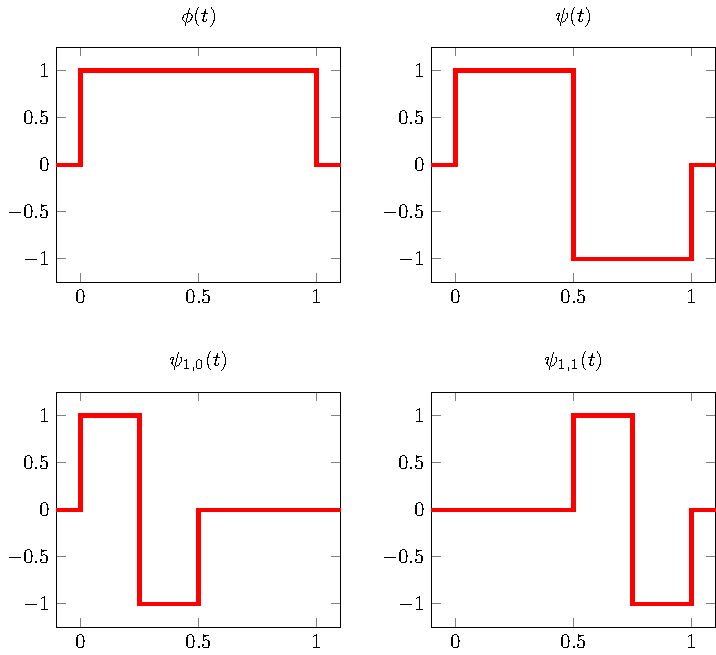
\includegraphics{figs/wavelets.pdf}
    \caption{First generation of Haar wavelet functions.}
    \label{fig:haar-fcn}
  \end{figure}

  \subsection{Child Wavelets}

  The Haar wavelet's support is the unit interval \([0,1]\). We can contract the mother function to get a wavelet half the size on the interval \([0,1/2]\), namely \(\psi(2t)\). Also, translating to fit the interval \([1/2,1]\), we get \(\psi(2t-1)\). See Figure \ref{fig:haar-fcn}. Since these smaller wavelets are derived from the mother, we call them daughter wavelets distinguishing them by parameters in subscripts, \(\psi_{1,0}(t) = \psi(2^1t-0) = \psi(2t)\) and \(\psi_{1,1}(t) = \psi(2^1t - 1) = \psi(2t-1)\). Likewise, son wavelets are derived from the father function.
  
  \section{Wavelet Basis}

  Our primary goal is to approximate a signal \(f(t)\) using wavelets. We will see that we are limited to signals with finite energy, that is \(f(t)\) must be in the Hilbert space
  \(L^2(\RR) = \left\{f \; \middle| \; f : \RR \to \RR, \int_{-\infty}^\infty f^2 < \infty\right\},\)
  the set of all square integrable functions.

  \subsection{Multiresolution Analysis}

  A nice feature of many wavelets, including the Haar, is the \textit{multiresolution analysis} (MRA) property, which provides a method to improve computational efficiency. First, consider the function space \(V_j = \spans\qty{\phi(2^jt-k) \mid k \in \ZZ}\) describing the subspace of \(L^2(\mathbb{R})\) generated by \(2^j\) resolution father functions. A function \(f \in L^2(\RR)\) can be approximated by the projection of \(f\) onto \(V_j\), that is
  \begin{equation} \label{eqn:proj-f-onto-vj}
    f_j(t) = \sum_{k \in \ZZ} h_k \phi(2^jt-k) \in V_j, 
    \qq{where}
    h_k = \iprod{f,\sqrt{2}\phi(2^jt-k)}.
  \end{equation}
  Notice that \(\phi(t)\) lives in the reference space \(V_0\). Then \(\phi(t)\) can be represented as a linear combination of functions in \(V_1\) and we have \(V_0 \subset V_1\). In general, we have a sequence of nested subspaces such that
  \begin{equation} \label{eqn:mra}
    \dots \subset V_{-1} \subset V_0 \subset V_1 \subset \dots \subset L^2(\mathbb{R}),
  \end{equation}
  forming a multiresolution analysis. In the case of the Haar wavelet, the MRA allows us to construct the mother function from our choice of the father function \(\phi(t) = 1\) on the unit interval and zero otherwise. Then \(W_j\) is generated by \(\qty{\psi(2^jt-k) \mid k \in \ZZ}\) such that \(V_{j+1} = V_j \oplus W_j\). In other words, \(W_j\) contains the information that is lost when a function is approximated at a lower resolution. For \(f_j \in V_j\) and \(w_j \in W_j\), the \(n\)-level decomposition of a function \(f_n \in V_n\) is given by
  \[f_n = f_{n-1} + w_{n-1} = f_{n-2} + w_{n-2} + w_{n-1} = \dots = f_0 + w_0 + w_1 + \dots + w_{n-1},\]
  where \(f_j\) and \(w_j\) are called the \textit{average details} and \textit{difference details}, respectively, at the \(j\)-th level.

  \subsection{Orthogonality of the Haar Wavelet}

  In the previous section, we constructed a spanning set using \(\phi(t)\) to approximate a function \(f(t) \in L^2(\RR)\). Using the relationship between the Haar wavelet functions, we see that \(\psi(t) = \phi(2t) - \phi(2t-1)\). Then it follows that we can construct a spanning set using \(\psi(t)\) such that
  \begin{equation} \label{eqn:proj-f-onto-wj}
    f(t) = \sum_{k \in \ZZ} g_k \psi(2^jt-k),
  \end{equation}
  where \(g_k\) are some scaling coefficients. Notice that as \(j\) increases, the spaces spanned by these sets approach \(L^2(\RR)\).

  By orthogonality, we can show that these spanning sets are linearly independent and, therefore, form an orthogonal basis. First, we see that the functions in \(V_j\) are disjoint and the functions in \(W_j\) are disjoint, so the pairwise inner products in each space are always zero. Also, if \(\phi_{j,k} \in V_j\) is translated by \(k\) and \(\psi_{j,k'} \in W_j\) is translated by \(k'\) with \(k \neq k'\), then \(\phi_{j,k}\) and \(\psi_{j,k'}\) are disjoint with an inner product of zero. So, suppose \(\phi_{j,k}\) and \(\psi_{j,k}\) have the same support, for example, consider \(\phi = \phi_{0,0}\) and \(\psi = \psi_{0,0}\) on the unit interval. Then
  \begin{equation*} \label{eqn:orthogonality-of-haar}
    \iprod{\phi,\psi}
      = \int_{-\infty}^\infty \phi(t) \overline{\psi(t)} \dd{t}
      = \int_{-\infty}^\infty \phi(t) \psi(t) \dd{t}
      = \int_{0}^{1/2}1 \dd{t} - \int_{1/2}^{1}1 \dd{t}
      = 0.
  \end{equation*}
  Other cases are similar, so we can conclude \(\iprod{\phi_{j,k},\psi_{j,k}} = 0\) for all \(j,k \in \ZZ\). Hence, the Haar wavelet functions \(\phi\) and \(\psi\) form an orthogonal basis under \(t \mapsto (2^jt-k)\) mappings.
  
  \subsection{Vector Representation}
  
  For computations, it is convenient to represent wavelets as vectors. For example, we can define the first generation of wavelet vectors as
  \begin{align*}
    \phi &\equiv (1,1,1,1), &
    \psi &\equiv (1,1,-1,-1), \\
    \psi_{1,0} &\equiv (1,-1,0,0), &
    \psi_{1,1} &\equiv (0,0,1,-1),
  \end{align*}
  which span \(\mathbb{R}^4\). Further, we can demonstrate that these vectors are mutually orthogonal by computing each of the inner products
  \begin{align*}
    \iprod{\psi, \phi} &=
    (1,1,-1,-1) (1,1,1,1)^T = 1+1-1-1 = 0, \\
    \iprod{\psi_{1,0}, \phi} &=
    (1,-1,0,0) (1,1,1,1)^T = 1-1+0+0 = 0, \\
    \iprod{\psi_{1,1}, \phi} &=
    (0,0,1,-1) (1,1,1,1)^T = 0+0+1-1 = 0, \\
    \iprod{\psi_{1,0}, \psi} &=
    (1,-1,0,0) (1,1,-1,-1)^T = 1-1+0+0 = 0, \\
    \iprod{\psi_{1,1}, \psi} &=
    (0,0,1,-1) (1,1,-1,-1)^T = 0+0-1+1 = 0, \\
    \iprod{\psi_{1,0}, \psi_{1,1}} &=
    (1,-1,0,0) (0,0,1,-1)^T = 0+0+0+0 = 0.
  \end{align*}
  As in the continuous case, we see that the wavelet vectors form an orthogonal basis. It will be especially useful to normalize these vectors so that the total energy of a function is not changed. Thus, when we divide by the norms \(\norm{\phi} = 2\), \(\norm{\psi} = 2\), \(\norm{\psi_{1,0}} = \sqrt{2}\), and \(\norm{\psi_{1,1}} = \sqrt{2}\), we obtain an orthonormal wavelet basis.
  
  \section{Decomposition and Reconstruction}

  In general, a wavelet decomposition is obtained using wavelet transforms. A series of inner products are computed using the signal function and wavelet for each level of the decomposition. However, thanks to MRA, these computations can be reduced for the Haar wavelet using a much more efficient algorithm. Moreover, we saw that the difference detail contains the lost information. Thus, the original signal can be perfectly reconstructed.

  The Haar wavelet transform \(\mathcal{H}_1\) decomposes a signal \(\vb{f}\) in \(\RR^n\) into the first average detail \(\vb{a}^1\) and first difference detail \(\vb{d}^1\) and we write
  \begin{equation}
    \vb{f} \xrightarrow{\mathcal{H}_1} (\vb{a}^1 \mid \vb{d}^1).
  \end{equation}

  \subsection{Decomposition Algorithm}

  Let \(\vb{f} = (f_1, f_2, \dots, f_n)\) be a signal with \(n\) even\footnote{If this is not the case, then a zero entry is appended to the signal.}. The average of the first two entries in \(\vb{f}\) is computed by
  \[a_1^1 = \frac{1}{\sqrt{2}} (1,1,0,0,\dots,0) \vb{f}^T = \frac{f_1 + f_2}{\sqrt{2}}.\]
  In general, the average detail of the \(m\)th pair of entries in \(\vb{f}\) is found using the formula
  \begin{equation} \label{eqn:avg-detail}
    a_m = \frac{f_{m-1} + f_{m}}{\sqrt{2}},
  \end{equation}
  for \(m = 1, 2, \dots, n/2\). Similarly, the difference detail is computed by
  \begin{equation} \label{eqn:diff-detail}
    d_m = \frac{f_{m-1} - f_{m}}{\sqrt{2}}.
  \end{equation}
  Then we obtain \(\vb{a}^1 = (a_1^1, a_2^1, \dots, a_{n/2}^1)\) and \(\vb{d}^1 = (d_1^1, d_2^1, \dots, d_{n/2}^1)\).

  \begin{example} \label{eg:decomp-1}
      Let \(\vb{f} = (-1, 1, 9, 4, 7, 6, -4, 10)\). We find the first average details using Equation \eqref{eqn:avg-detail}
      \begin{align*}
      a_1^1 &= \frac{-1+1}{\sqrt{2}} = \frac{0}{\sqrt{2}}, &
      a_2^1 &= \frac{9+4}{\sqrt{2}} = \frac{13}{\sqrt{2}},\\
      a_3^1 &= \frac{7+6}{\sqrt{2}} = \frac{13}{\sqrt{2}}, &
      a_4^1 &= \frac{-4+10}{\sqrt{2}} = \frac{6}{\sqrt{2}},
    \end{align*}
    and the first difference details using Equation \eqref{eqn:diff-detail}
    \begin{align*}
      d_1^1 &= \frac{-1-1}{\sqrt{2}} = \frac{-2}{\sqrt{2}}, &
      d_2^1 &= \frac{9-4}{\sqrt{2}} = \frac{5}{\sqrt{2}},\\
      d_3^1 &= \frac{7-6}{\sqrt{2}} = \frac{1}{\sqrt{2}}, &
      d_4^1 &= \frac{-4-10}{\sqrt{2}} = \frac{-14}{\sqrt{2}}.
    \end{align*}
    Then we have
    \begin{align*}
      \vb{a}^1 &= \frac{1}{\sqrt{2}}(0,13,13,6), &
      \vb{d}^1 &= \frac{1}{\sqrt{2}}(-2,5,1,-14).
    \end{align*}
  \end{example}

  \subsection{Matrix Representation of the Decomposition}

  Instead of using Equations \eqref{eqn:avg-detail} and \eqref{eqn:diff-detail} iteratively to compute the average and difference detail, we can combine the steps using matrices.
  For a given signal \(\vb{f}\) of length \(n\), we use the son wavelets to get
  \begin{equation}
    H = \frac{1}{\sqrt{2}}
    \begin{pmatrix}
      1 & 1 & 0 & 0 & \cdots & 0\\
      0 & 0 & 1 & 1 & \cdots & 0\\
      \vdots & \vdots &  & \ddots & \ddots & \vdots\\
      0 & 0 & \multicolumn{2}{c}{\cdots} & 1 & 1
    \end{pmatrix}
  \end{equation}
  and the daughter wavelets to get
  \begin{equation}
    G = \frac{1}{\sqrt{2}}
    \begin{pmatrix}
      1 & -1 & 0 & 0 & \cdots & 0\\
      0 & 0 & 1 & -1 & \cdots & 0\\
      \vdots & \vdots &  & \ddots & \ddots & \vdots\\
      0 & 0 & \multicolumn{2}{c}{\cdots} & 1 & -1
    \end{pmatrix},
  \end{equation}
  where \(H\) and \(G\) each have \(n/2\) rows and \(n\) columns. Now, we can write the Haar wavelet decomposition as \(\vb{a}^1 = H \vb{f}\) and \(\vb{d}^1 = G\vb{f}\) to get the matrix equation
  \begin{equation}
    \begin{pmatrix}
      \vb{a}^1 \\ \vb{d}^1
    \end{pmatrix} =
    \begin{pmatrix}
      H\vb{f} \\ G\vb{f}
    \end{pmatrix} =
    \begin{pmatrix}
      H \\ G
    \end{pmatrix} \vb{f}.
  \end{equation}
  Since \(H\) and \(G\) were constructed from an orthonormal Haar wavelet basis, the matrix \(\smqty(H \\ G)\) is orthonormal as well. Then left-hand multiplication by \(\smqty(H \\ G)^T\) will allow us to solve for \(\vb{f}\), and we get
  \begin{equation}
    \vb{f} =
    \begin{pmatrix}
      H \\ G
    \end{pmatrix}^T
    \begin{pmatrix}
      \vb{a}^1 \\ \vb{d}^1
    \end{pmatrix} =
      (H^T \mid G^T)
    \begin{pmatrix}
      \vb{a}^1 \\ \vb{d}^1
    \end{pmatrix} =
    H^T \vb{a}^1 + G^T \vb{d}^1.
  \end{equation}
  Therefore, we say that the signal is reconstructed by the inverse Haar wavelet transform
  \begin{equation}
    (\vb{a}^1 \mid \vb{d}^1)  \xrightarrow{\mathcal{H}^{-1}_1} \vb{f}.
  \end{equation}

  \begin{example}
    Let \(\vb{a}^1\) and \(\vb{d}^1\) be given from Example \ref{eg:decomp-1} as
    \begin{align*}
      \vb{a}^1 &= \left(
        0,
        \frac{13}{\sqrt{2}},
        \frac{13}{\sqrt{2}},
        \frac{6}{\sqrt{2}}
      \right), &
      \vb{d}^1 &= \left(
        \frac{-2}{\sqrt{2}},
        \frac{5}{\sqrt{2}},
        \frac{1}{\sqrt{2}},
        \frac{-14}{\sqrt{2}}
      \right).
    \end{align*}
    To reconstruct \(\vb{f}\) we compute \(H^T\vb{a}^1\) and \(G^T\vb{d}^1\).
    \begin{align*}
      H^T\vb{a}^1 &= \frac{1}{\sqrt{2}}
      \begin{pmatrix}
        1 & 0 & 0 & 0\\
        1 & 0 & 0 & 0\\
        0 & 1 & 0 & 0\\
        0 & 1 & 0 & 0\\
        0 & 0 & 1 & 0\\
        0 & 0 & 1 & 0\\
        0 & 0 & 0 & 1\\
        0 & 0 & 0 & 1
      \end{pmatrix} \cdot \frac{1}{\sqrt{2}}
      \begin{pmatrix}
        0 \\
        13 \\
        13 \\
        6
      \end{pmatrix} = \frac{1}{2}
      \begin{pmatrix}
        0 \\
        0 \\
        13 \\
        13 \\
        13 \\
        13 \\
        6 \\
        6 \\
      \end{pmatrix}\\
      G^T\vb{d}^1 &= \frac{1}{\sqrt{2}}
      \begin{pmatrix}
        1 & 0 & 0 & 0\\
        -1 & 0 & 0 & 0\\
        0 & 1 & 0 & 0\\
        0 & -1 & 0 & 0\\
        0 & 0 & 1 & 0\\
        0 & 0 & -1 & 0\\
        0 & 0 & 0 & 1\\
        0 & 0 & 0 & -1
      \end{pmatrix} \cdot \frac{1}{\sqrt{2}}
      \begin{pmatrix}
        -2 \\
        5 \\
        1 \\
        -14
      \end{pmatrix} = \frac{1}{2}
      \begin{pmatrix}
        -2 \\
        2 \\
        5 \\
        -5 \\
        1 \\
        -1 \\
        -14 \\
        14 \\
      \end{pmatrix}
    \end{align*}
    Then we have
    \[\vb{f} = H^T \vb{a}^1 + G^T \vb{d}^1 = \frac{1}{2}
    \begin{pmatrix}
      0 \\ 0 \\ 13 \\ 13 \\ 13 \\ 13 \\ 6 \\ 6
    \end{pmatrix} + \frac{1}{2}
    \begin{pmatrix}
      -2 \\ 2 \\ 5 \\ -5 \\ 1 \\ -1 \\ -14 \\ 14
    \end{pmatrix} = \frac{1}{2}
    \begin{pmatrix}
      -2 \\ 2 \\ 18 \\ 8 \\ 14 \\ 12 \\ -8 \\ 20
    \end{pmatrix} =
    \begin{pmatrix}
      -1 \\ 1 \\ 9 \\ 4 \\ 7 \\ 6 \\ -4 \\ 10
    \end{pmatrix}.\]
  \end{example}

  \subsection{Multi-Level Decomposition}
  After obtaining a decomposed signal \((\vb{a}^1 \mid \vb{d}^1)\), we can continue breaking the average detail into smaller components. Using the second level Haar wavelet transform, we have
  \begin{equation*}
    \vb{f} \xrightarrow{\mathcal{H}_1} (\vb{a}^1 \mid \vb{d}^1) \xrightarrow{\mathcal{H}_2} (\vb{a}^2 \mid \vb{d}^2 \mid \vb{d}^1).
  \end{equation*}
  Using appropriately-sized matrices \(H\) and \(G\), we decompose the first-level average detail \(\vb{a}^1\) into \((\vb{a}^2 \mid \vb{d}^2)\).

  % \begin{example}
  %   From Example \ref{eg:decomp-1} we computed \(\vb{a}^1 =
  %   \begin{pmatrix}
  %     0 &
  %     \frac{13}{\sqrt{2}} &
  %     \frac{13}{\sqrt{2}} &
  %     \frac{6}{\sqrt{2}}
  %   \end{pmatrix}\). Then applying the level-two decomposition, we have
  %   \begin{align*}
  %     a_1^2 &= \frac{0 + \frac{13}{\sqrt{2}}}{\sqrt{2}} = \frac{13}{2}, &
  %     a_2^2 &= \frac{\frac{13}{\sqrt{2}} + \frac{6}{\sqrt{2}}}{\sqrt{2}} = \frac{19}{2}, \\
  %     d_1^2 &= \frac{0 - \frac{13}{\sqrt{2}}}{\sqrt{2}} = \frac{-13}{2}, &
  %     d_2^2 &= \frac{\frac{13}{\sqrt{2}} - \frac{6}{\sqrt{2}}}{\sqrt{2}} = \frac{7}{2}.
  %   \end{align*}
  % \end{example}

  \subsection{Two-Dimensional Haar Wavelet Transform}
  The idea of signal decomposition using the Haar wavelet can be extended so that we can transform a matrix \(\vb{f}\) into first-level details. Then we have
  \begin{equation} 
    \vb{f} \xrightarrow{\mathcal{H}_1}
    \left(\begin{array}{c|c}
      \vb{a}^1 & \vb{h}^1\\ \hline
      \vb{v}^1 & \vb{d}^1
    \end{array}\right),
  \end{equation}
  where \(\vb{h}^1\) is the horizontal difference detail, \(\vb{v}^1\) is the vertical difference detail, and \(\vb{d}^1\) is the diagonal difference detail. If \(\vb{f}\) is an \(m \times n\) signal matrix, for \(m\) and \(n\) even\footnote{If this is not the case, then add a row and/or column of zeros to \(\vb{f}\) to make the dimensions even.}, then the first-level details can be computed using a similar matrix algorithm to obtain
  \begin{align} \label{eqn:matrix-decomp}
      \vb{a}^1 &= H \vb{f} H^T, &
      \vb{h}^1 &= H \vb{f} G^T, &
      \vb{v}^1 &= G \vb{f} H^T, &
      \vb{d}^1 &= G \vb{f} G^T,
  \end{align}
  where \(H\) and \(G\) on the left are sized \(m/2 \times m\) and \(H^T\) and \(G^T\) on the right are sized \(n \times n/2\) so that multiplication is defined.
  
  \begin{example} \label{eg:image-matrix-4}
    Consider the \(4 \times 4\) grayscale image with intensity values ranging from 0 (black) to 255 (white) represented as a matrix \(\vb{f}\).
    \[
      \vb{f} =
      \begin{pmatrix}
        67 & 148 & 159 & 19 \\
        37 & 140 & 89 & 61 \\
        35 & 37 & 131 & 31 \\
        22 & 218 & 102 & 47
      \end{pmatrix}
      \quad
      \longleftrightarrow
      \quad
      \begin{gathered}
      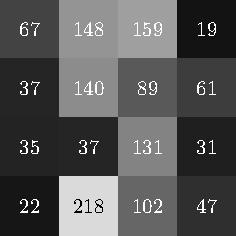
\includegraphics[scale=.75]{figs/fig-image-4.pdf}
      \end{gathered}
    \]
    The average detail \(\vb{a}^1\) is found in two steps. First we compute detail from the columns by the left-hand multiplication
    \begin{align*}
      H \vb{f} &= \frac{1}{\sqrt{2}}
      \begin{pmatrix}
        1 & 1 & 0 & 0\\
        0 & 0 & 1 & 1
      \end{pmatrix}
      \begin{pmatrix}
        67 & 148 & 159 & 19 \\
        37 & 140 & 89 & 61 \\
        35 & 37 & 131 & 31 \\
        22 & 218 & 102 & 47
      \end{pmatrix}\\
      &= \frac{1}{\sqrt{2}}
      \begin{pmatrix}
        67 + 37 & 148 + 140 & 159 + 89 & 19 + 61\\
        35 + 22 & 37 + 218 & 131 + 102 & 31 + 47
      \end{pmatrix}\\
      &= \frac{1}{\sqrt{2}}
      \begin{pmatrix}
        104 & 288 & 248 & 80 \\
        57 & 255 & 233 & 78
      \end{pmatrix}
    \end{align*}
    Then we find \(\vb{a}^1\) by the right-hand multiplication
    \begin{align*} % average detail
      \vb{a}^1 = (H \vb{f}) H^T &= \frac{1}{\sqrt{2}}
      \begin{pmatrix}
        104 & 288 & 248 & 80 \\
        57 & 255 & 233 & 78
      \end{pmatrix}
      \cdot \frac{1}{\sqrt{2}}
      \begin{pmatrix}
        1 & 0\\
        1 & 0\\
        0 & 1\\
        0 & 1
      \end{pmatrix}\\
      &= \frac{1}{2}
      \begin{pmatrix}
        104 + 288 & 248 + 80 \\
        57 + 255 & 233 + 78
      \end{pmatrix}\\
      &= \frac{1}{2}
      \begin{pmatrix}
        392 & 328\\
        312 & 311
      \end{pmatrix}
    \end{align*}
    Similarly, we can find \(\vb{h}^1\), \(\vb{v}^1\), and \(\vb{d}^1\) to get
    \begin{align*}
    % average detail
      \vb{a}^1 &=
      \frac{1}{2}
      \begin{pmatrix}
        392 & 328\\
        312 & 311
      \end{pmatrix},&
    % horizontal detail
      \vb{h}^1 &= H\vb{f}G^T
      = \frac{1}{2}
      \begin{pmatrix}
        -184 & 168 \\
        -198 & 155
      \end{pmatrix},\\
    % vertical detail
      \vb{v}^1 &= G\vb{f}H^T
      = \frac{1}{2}
      \begin{pmatrix}
          38 & 28 \\
        -168 & 13
      \end{pmatrix},&
    % diagonal detail
      \vb{d}^1 &= G\vb{f}G^T
      = \frac{1}{2}
      \begin{pmatrix}
         22 & 112 \\
        194 &  45
      \end{pmatrix}.
    \end{align*}
    Finally, we write the decomposition as
    \[
      \frac{1}{2}
      \left(
        \begin{array}{rr|rr}
          392 & 328 & -184 & 168 \\
          312 & 311 & -198 & 155 \\
          \hline
          38 &  28 &   22 & 112 \\
          -168 &  13 &  194 &  45
        \end{array}
      \right) =
      \left(
        \begin{array}{rr|rr}
          196 &   164\phantom{.5} & -92 &   84\phantom{.5} \\
          156 & 155.5 & -99 & 77.5 \\
          \hline
           19 &    14\phantom{.5} &  11 &   56\phantom{.5} \\
          -84 &   6.5 &  97 & 22.5
        \end{array}
      \right).
    \]
  \end{example}

  % Reconstruction is obtained by the two-dimensional inverse Haar transform. Since \((\begin{smallmatrix}
  %   H \\ G
  % \end{smallmatrix})\) and \((\begin{smallmatrix}
  %   H \\ G
  % \end{smallmatrix})^T\) are orthonormal matrices, we have
  % \begin{equation*}
  %   \begin{pmatrix}
  %     H \\ G
  %   \end{pmatrix} \vb{f}
  %   \begin{pmatrix}
  %     H^T & G^T
  %   \end{pmatrix} =
  %   \begin{pmatrix}
  %     Hf \\ Gf
  %   \end{pmatrix}
  %   \begin{pmatrix}
  %     H^T & G^T
  %   \end{pmatrix} =
  %   \begin{pmatrix}
  %     HfH^T & HFG^T \\
  %     GfH^T & GfG^T
  %   \end{pmatrix} =
  %   \begin{pmatrix}
  %     \vb{a}^1 & \vb{h}^1\\
  %     \vb{v}^1 & \vb{d}^1
  %   \end{pmatrix}.
  % \end{equation*}
  % Then
  % \begin{align*}
  %   \vb{f} &=
  %   \begin{pmatrix}
  %     H \\ G
  %   \end{pmatrix}^T
  %   \begin{pmatrix}
  %     \vb{a}^1 & \vb{h}^1\\
  %     \vb{v}^1 & \vb{d}^1
  %   \end{pmatrix}
  %   \begin{pmatrix}
  %     H^T & G^T
  %   \end{pmatrix}^T \\ &=
  %   \begin{pmatrix}
  %     H^T & G^T
  %   \end{pmatrix}
  %   \begin{pmatrix}
  %     \vb{a}^1 & \vb{h}^1\\
  %     \vb{v}^1 & \vb{d}^1
  %   \end{pmatrix}
  %   \begin{pmatrix}
  %     H \\ G
  %   \end{pmatrix} \\ &=
  %   \begin{pmatrix}
  %     H^T\vb{a}^1 + G^T\vb{v}^1 &
  %     H^T\vb{h}^1 + G^T\vb{d}^1
  %   \end{pmatrix}
  %   \begin{pmatrix}
  %     H \\ G
  %   \end{pmatrix} \\ &=
  %   \begin{pmatrix}
  %     H^T\vb{a}^1 + G^T\vb{v}^1
  %   \end{pmatrix} H +
  %   \begin{pmatrix}
  %     H^T\vb{h}^1 + G^T\vb{d}^1
  %   \end{pmatrix} G \\ &=
  %   H^T \vb{a}^1 H +
  %   G^T \vb{v}^1 H +
  %   H^T \vb{h}^1 G +
  %   G^T \vb{d}^1 G.
  % \end{align*}
  % This results in a convenient formula for reconstructing a signal from its decomposed form, that is,
  % \begin{equation}
  %   \vb{f} =
  %   H^T \vb{a}^1 H +
  %   H^T \vb{h}^1 G +
  %   G^T \vb{v}^1 H +
  %   G^T \vb{d}^1 G.
  % \end{equation}

  % To complete the previous example,
  % \begin{align*}
  %   \vb{f} &=
  %   H^T \begin{pmatrix}
  %     196 & 164\\
  %     156 & 155.5
  %   \end{pmatrix} H +
  %   H^T \begin{pmatrix}
  %     -92 & 84\\
  %     -99 & 77.5
  %   \end{pmatrix} G \\ &\qquad +
  %   G^T \begin{pmatrix}
  %     19 & 14\\
  %     -84 & 6.5
  %   \end{pmatrix} H +
  %   G^T \begin{pmatrix}
  %     11 & 56\\
  %     97 & 22.5
  %   \end{pmatrix} G.
  % \end{align*}
  % This gives
  % \begin{align*}
  %   \vb{f} &= \frac{1}{2}
  %   \begin{pmatrix}
  %     196 & 196 & 164 & 164 \\
  %     196 & 196 & 164 & 164 \\
  %     156 & 156 & 155.5 & 155.5 \\
  %     156 & 156 & 155.5 & 155.5
  %   \end{pmatrix} + \frac{1}{2}
  %   \begin{pmatrix}
  %     -92 & 92 & 84 & -84 \\
  %     -92 & 92 & 84 & -84 \\
  %     -99 & 99 & 77.5 & -77.5 \\
  %     -99 & 99 & 77.5 & -77.5
  %   \end{pmatrix} \\ &\qquad + \frac{1}{2}
  %   \begin{pmatrix}
  %     19 & 19 & 14 & 14 \\
  %     -19 & -19 & -14 & -14 \\
  %     -84 & -84 & 6.5 & 6.5 \\
  %     84 & 84 & -6.5 & -6.5
  %   \end{pmatrix} + \frac{1}{2}
  %   \begin{pmatrix}
  %     11 & -11 & 56 & -56 \\
  %     -11 & 11 & -56 & 56 \\
  %     97 & -97 & 22.5 & -22.5 \\
  %     -97 & 97 & -22.5 & 22.5
  %   \end{pmatrix} \\ &= \frac{1}{2}
  %   \begin{pmatrix}
  %     196-92+19+11 & 196+92+19-11 & \cdots\\
  %     196-92-19-11 & 196+92-19+11 & \cdots\\
  %     \vdots & \vdots & \ddots
  %   \end{pmatrix} \\ &=
  %   \begin{pmatrix}
  %     67 & 148 & 159 & 19 \\
  %     37 & 140 & 89 & 61 \\
  %     35 & 37 & 131 & 31 \\
  %     22 & 218 & 102 & 47
  %   \end{pmatrix}.
  % \end{align*}

  \section{Image Compression}

  When applying \(k\) multi-level Haar transforms, the dimensions of the decomposed matrix are the same as the original signal matrix. Since no information has been lost, the signal can always be perfectly reconstructed. This also means that the file size stored in memory has not been reduced.
  
  \subsection{Thresholding}
  Wavelet transforms like the Haar are well-suited for image compression because they preserve low-frequency information, such as general shapes and boundaries, while the high-frequency noise is mapped into small difference details. If the magnitude of the difference is small enough, say less than some parameter \(\lambda\), then we can set the value to zero. This is known as thresholding, which handles the actual compression. A larger threshold value \(\lambda\) gives better compression, however, if \(\lambda\) is too large, then much of the image quality will be lost.
  We represent thresholding as the transform
  \begin{equation} \label{eqn:threshold}
    T(x;\lambda) = \begin{cases}
      0, & |x| \leq \lambda,\\
      x, & |x| > \lambda,
    \end{cases}
  \end{equation}
  where \(x\) is an element of the \(k\)-level wavelet decomposition of a signal \(\vb{f}\). Since \(T\) maps a range of values \(- \lambda \leq x \leq \lambda\) to zero, the function is not one-to-one. Thus, when applying a threshold transform, we no longer have perfect reconstruction, but sparsity of the image matrix increases. This corresponds to a reduction in file size as desired.

  In particular, Equation \eqref{eqn:threshold} is known as hard thresholding. Other types of thresholding (e.g. soft) are common and use neighboring pixels to blend the image. This leads to a variety of wavelet applications in denoising images and data.

  \subsection{Method}
  In MATLAB, we can import a color image as a 3-dimensional array with the command \mintinline{matlab}{imread('filename.png')} in RGB or YCbCr color space\footnote{For wavelet decomposition, YCbCr is preferred since RGB layers are usually correlated. So, an image is converted using \mintinline{matlab}{rgb2ycbcr(image)}.}.
  
  Using the Wavelet Toolbox, we perform the two-dimensional decomposition of each image layer with \mintinline{matlab}{wavedec2(x,k,wname)}. This function requires three parameters: a 2-dimensional array representing the image color layer, an integer representing the number of levels of decomposition, and a string representing the name of the wavelet. For our purposes, we will use \mintinline{matlab}{'haar'} for the wavelet name and the maximum level of decompositions, \(\texttt{k} = \floor(\log_2(\min\qty{m,n}))\), where the image dimensions are \(m\) pixels by \(n\) pixels. The outputs for each layer will be a decomposition vector \mintinline{matlab}{C} and a coefficient matrix \mintinline{matlab}{S}.

  The compression is handled by \mintinline{matlab}{wdencmp('gbl',C,S,wname,k,thr,sorh,1)}. Parameters \mintinline{matlab}{C} and \mintinline{matlab}{S} are passed in from the \mintinline{matlab}{wavedec2} outputs, \mintinline{matlab}{wname} and \mintinline{matlab}{k} are reused, \mintinline{matlab}{thr} is the thresholding value, and \mintinline{matlab}{sorh} is either \mintinline{matlab}{'s'} (for soft thresholding) or \mintinline{matlab}{'h'} (for hard thresholding).

  Lastly, the image is reconstructed by creating 3-dimensional array from the outputs of \mintinline{matlab}{wdencmp()} performed on each color layer. This process is summarized in Figure \ref{fig:process-diagram}.

  \begin{figure}
    \centering
    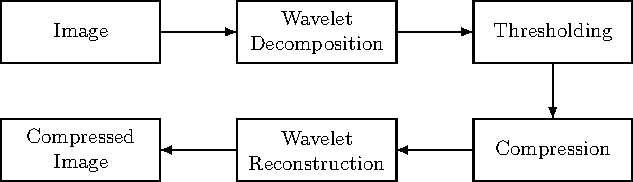
\includegraphics{figs/fig-process.pdf}
    \caption{Wavelet image compression process diagram.}
    \label{fig:process-diagram}
  \end{figure}

  \subsection{Performance}
  The compression ratio (CR) is computed by comparing the original image file size to the compressed image file size. Using various threshold values \(\lambda\), we compress standard test images, Lena and Peppers, with the Haar wavelet in MATLAB with hard thresholding in YCbCr color space. The results are in Table \ref{tab:compression-ratio} and corresponding Figures
  \ref{fig:lena} and \ref{fig:peppers}.
  \begin{table}[ht]
    \centering
    \begin{tabular}{c|c|c|c|c}
      Image & \(\lambda\) & Orig. Size & Comp. Size & CR\\
      \hline
      Lena & 5 & 465.09 KB & 272.53 KB & 1.7\\
      $\cdots$ & 10 & $\cdots$ & 150.63 KB & 3.1\\
      $\cdots$ & 20 & $\cdots$ & 86.794 KB & 5.4\\
      \hline
      Peppers & 5 & 280.85 KB & 122.40 KB & 2.3\\
      $\cdots$ & 10 & $\cdots$ & 81.078 KB & 3.5\\
      $\cdots$ & 20 & $\cdots$ & 51.649 KB & 5.4
    \end{tabular}
    \caption{Compression ratio for test images.}
    \label{tab:compression-ratio}
  \end{table}

  \clearpage
  \newgeometry{left=.5in,right=.5in}

  \begin{figure}
    \centering
    \begin{subfigure}[t]{.49\linewidth}
      \centering
      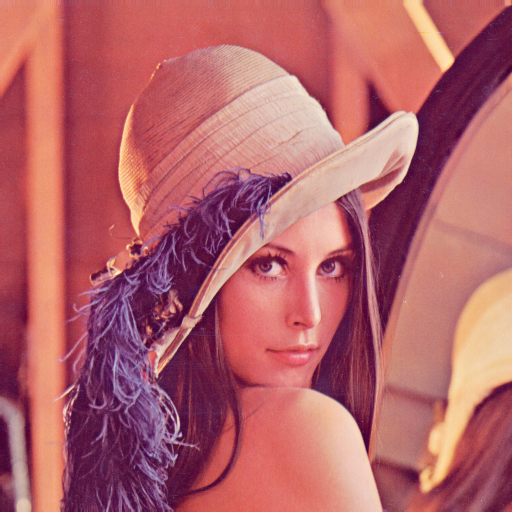
\includegraphics[width=.93\linewidth]{figs/lena.png}
      \caption{Original (465.09 KB)}
    \end{subfigure}
    \begin{subfigure}[t]{.49\linewidth}
      \centering
      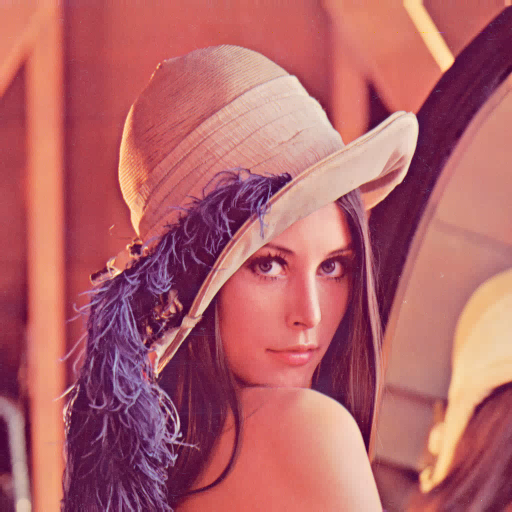
\includegraphics[width=.93\linewidth]{figs/lena_haar_5.png}
      \caption{Compressed \(\lambda = 5\) (272.53 KB)}
    \end{subfigure}
    \begin{subfigure}[t]{.49\linewidth}
      \centering
      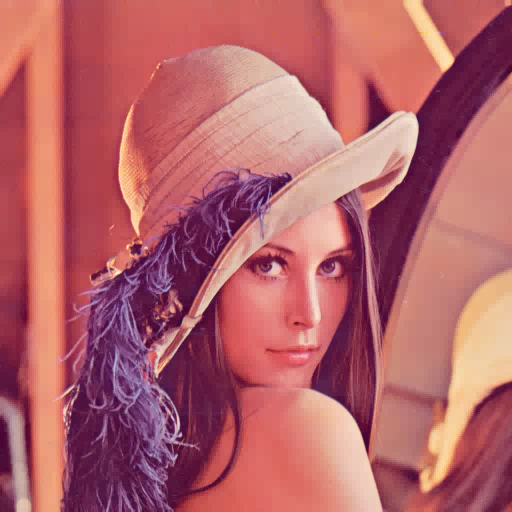
\includegraphics[width=.93\linewidth]{figs/lena_haar_10.png}
      \caption{Compressed \(\lambda = 10\) (150.63 KB)}
    \end{subfigure}
    \begin{subfigure}[t]{.49\linewidth}
      \centering
      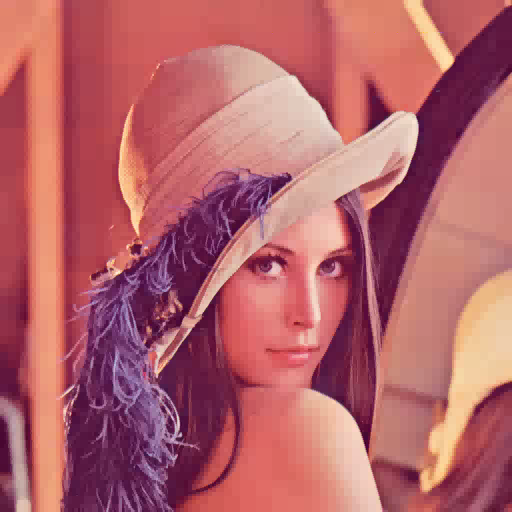
\includegraphics[width=.93\linewidth]{figs/lena_haar_20.png}
      \caption{Compressed \(\lambda = 20\) (86.794 KB)}
    \end{subfigure}
    \caption{Lena image comparison.}
    \label{fig:lena}
  \end{figure}

  \clearpage

  \begin{figure}
    \centering
    \begin{subfigure}[t]{.49\linewidth}
      \centering
      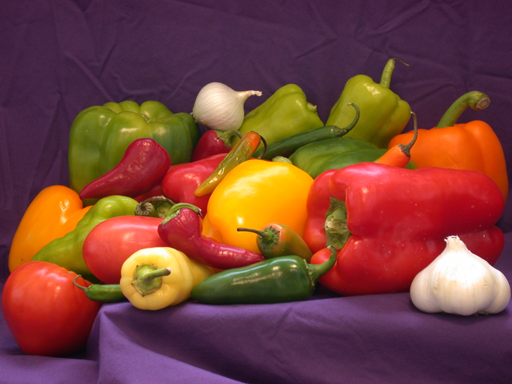
\includegraphics[trim={0 0 3.7in 2.8in},clip]{figs/peppers.png}
      \caption{Original (280.85 KB)}
    \end{subfigure}
    \begin{subfigure}[t]{.49\linewidth}
      \centering
      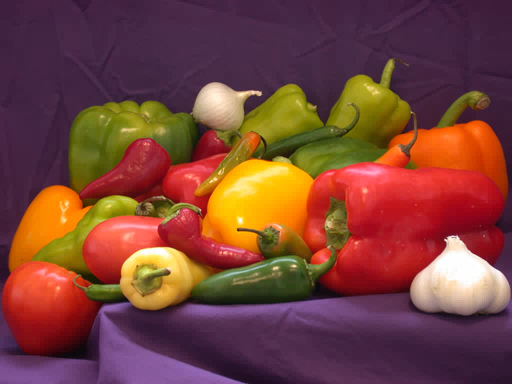
\includegraphics[trim={0 0 3.7in 2.8in},clip]{figs/peppers_haar_5.png}
      \caption{Compressed \(\lambda = 5\) (122.40 KB)}
    \end{subfigure}
    \begin{subfigure}[t]{.49\linewidth}
      \centering
      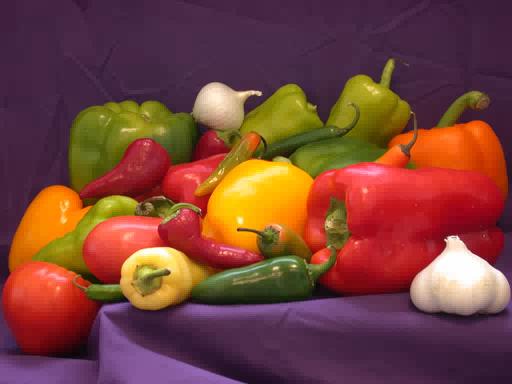
\includegraphics[trim={0 0 3.7in 2.8in},clip]{figs/peppers_haar_10.png}
      \caption{Compressed \(\lambda = 10\) (81.078 KB)}
    \end{subfigure}
    \begin{subfigure}[t]{.49\linewidth}
      \centering
      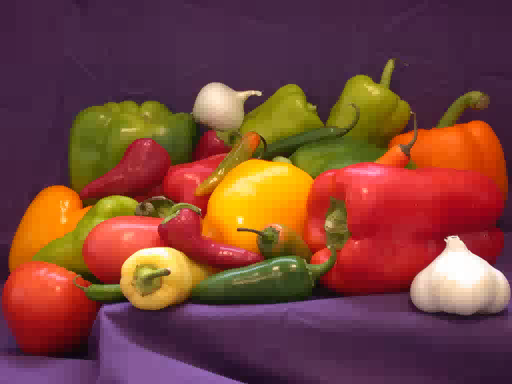
\includegraphics[trim={0 0 3.7in 2.8in},clip]{figs/peppers_haar_20.png}
      \caption{Compressed \(\lambda = 20\) (51.649 KB)}
    \end{subfigure}
    \caption{Peppers image comparison with details.}
    \label{fig:peppers}
  \end{figure}
  \clearpage
  \restoregeometry

  \nocite{*}

  \bibliographystyle{plain}
  \bibliography{refs}

\end{document}